\section{Theorie}
\label{sec:Theorie}

Zunächst wird allgemein auf Polarisation von Wellen eingegangen.
Dann wird sich mit dem prinzipiellen Aufbau eines Lasers beschäftigt und wie dieser kohärentes Licht produziert.
Anschließend \textit{tbd}.

\subsection{Polarisation und Kohärenz} \label{sec:polarisation}
Seit der Elektrodynamik ist bekannt, dass Licht als eine elektromagnetische Welle beschrieben werden kann.
\textbf{Kohärentes Licht} beschreibt Licht mit fester Frequenz, Phase und Ausbreitungsrichtung und kann mithilfe von Lasern erzeugt werden.
Nun ist bei verschiedenen physikalischen Prozessen auch die sogenannte \textbf{Polarisation} wichtig.
Eine polarisierte Welle ist in \autoref{fig:polarisation1} dargestellt.
Eine polarisierte Welle schwingt nur in einer Ebene in Bewegungsrichtung.
Beispielweise bei Interferenzphänomenen müssen zwei Lichtwellen in einer Ebene polarisiert sein, damit sie interferieren können.
\begin{figure}
    \centering
    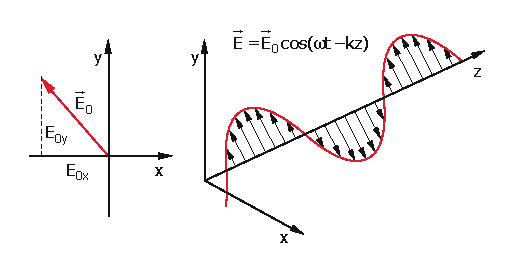
\includegraphics[width = 0.7 \linewidth]{pictures/polarisation1.pdf}
    \caption{Eine linear polarisierte Welle \cite{demtroeder2}.}
    \label{fig:polarisation1}
\end{figure}
\subsection{Aufbau eines Lasers}
\label{sec:aufbau1} 
\begin{figure}
    \centering
    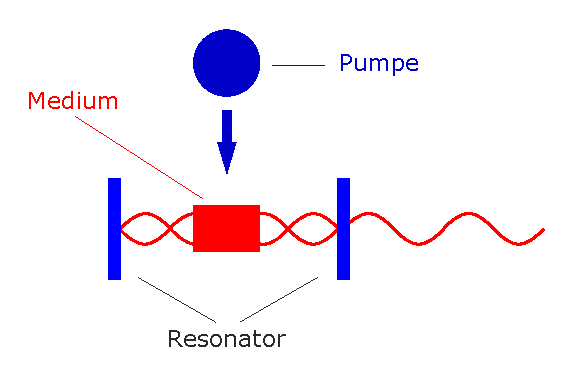
\includegraphics[width = 0.7 \linewidth]{pictures/aufbau1.pdf}
    \caption{Schematischer Aufbau eines Lasers \cite{leifilaser}.}
    \label{fig:aufbau1}
\end{figure}
Wie bereits angemerkt, produziert ein Laser (Light Amplification by Stimulated Emission Radiation) kohärentes Licht.
Im folgenden soll darauf eingegangen werden wie kohärentes Licht in einem Laser produziert wird.
Schematisch ist der Aufbau eines Lasers in \autoref{fig:aufbau1} dargestellt.
Grundlegend besteht ein Laser immer aus drei Komponenten.
Diese Komponenten sind ein sogenanntes \textbf{aktives Medium}, ein \textbf{Resonator} und eine \textbf{Pumpquelle}.
\subsubsection*{Aktives Medium}
\begin{wrapfigure}{r}{0.5\textwidth}
    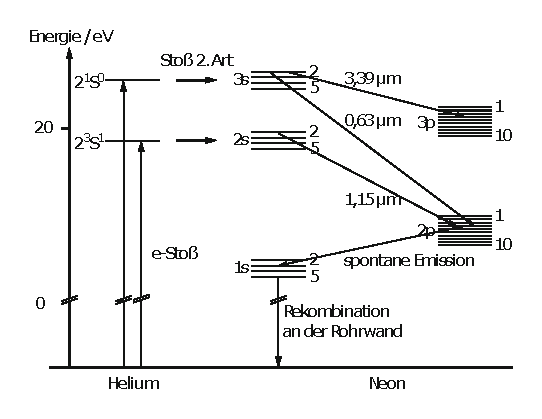
\includegraphics{pictures/HeNe_levels.pdf}
    \caption{Schematischer Aufbau eines Lasers \cite{HeNe_levels}.}
    \label{fig:HeNe_levels}
\end{wrapfigure}
Unter einem aktiven Medium wird ein verstanden, dass es durch \textbf{Besetzungsinversion} und \textbf{stimulierter Emission} kohärentes Licht abgibt \cite{demtroeder_laser}.
In einem Laser wird dies dann so angeordnet, dass es immer weiter verstärkt wird.
Ein Material ist dann ein geeigneter Kandidat für ein aktives Medium, wenn es über ein 3-Niveau-System\footnote{Aufgrund der Notwendigkeit eines metastabilen Zwischenzustandes, ist ein 2-Niveau-System nicht möglich.} verfügt.
Dann lässt sich mit der stimulierten Emission die Abstrahlung des Photons bei Anregung verstärken.
Da Medium kann dabei fest, flüssig oder auch gasförmig sein.
Dies geschieht dadurch, dass das angeregte Photon mit einem weiteren Photon angestrahlt wird und dann durch quantenmechanische Effekte beim Abstrahlen quasi kopiert wird (kohärent).
Dieser Prozess wird als Besetzungsinversion bezeichnet, da sich dann mehr Elektronen in einem höheren Energiezustand befinden als im Grundzustand.
Das aktive Lasermedium legt also auch die Wellenlänge fest, da es sich um die charakteristischen Photonen des jeweiligen Materials handelt.
Die Niveaus, die in einem HeNe Laser durchlaufen werden, sind in \autoref{fig:HeNe_levels} dargestellt.
Bei einem Helium-Neon Laser (HeNe) liegt diese Wellenlänge bei $632.8 \unit{\nano\meter}$.
\subsubsection*{Pumpquelle}
Die Pumpquelle ist in erster Linie dafür verantwortlich, Energie in das aktive Medium zu bringen.
Dies kann durch Licht, aber auch durch andere Prozesse geschehen.
Ohne dieses Pumpen, kann keine Besetzungsinversion vorliegen.